%
%%%%%%%%%%%%%%%%%%%%%%%%%%%%%%%%%%%%%%%%%%%%%%%%%%%%%%%%%%%%%%%%%%%%%%%%%%%%%%%%
\chapter{Theoretical background}\label{chap:1}
%%%%%%%%%%%%%%%%%%%%%%%%%%%%%%%%%%%%%%%%%%%%%%%%%%%%%%%%%%%%%%%%%%%%%%%%%%%%%%%%
%

%
%%%%%%%%%%%%%%%%%%%%%%%%%%%%%%%%%%%%%%%%%%%%%%%%%%%%%%%%%%%%%%%%%%%%%%%%%%%%%%%%
\section{Introduction}\label{sec:intro}
%%%%%%%%%%%%%%%%%%%%%%%%%%%%%%%%%%%%%%%%%%%%%%%%%%%%%%%%%%%%%%%%%%%%%%%%%%%%%%%%
%
Many crystals with a lack of inversion symmetry show an interesting phase
consisting of a regular arrangement of magnetic whirl tubes called skyrmions.
These spin configurations are found in a wide range of  chiral
magnets~\cite{skyrm1, skyrm2, skyrm3, skyrm4, skyrm5, skyrm6, Milde, skyrm8,
skyrm9, skyrm10} and have received a lot of attentian lately mostly due to the
topological stability of a quantized winding number associated with the whirl
tubes. Defect mobility or skyrmion switching~\cite{switch} might make them
suitable candidates for a permanent fast and efficient memory or other
spintronic devices.

Besides direct observation through a variety of experimental techniques, numeric
simulations have contributed significantly to the understanding of
skyrmions~\cite{skyrmion, Milde, switch}. The typical setup is a
three-dimensional spin lattice with a discretized Hamiltonian consisting of
direct exchange, an external field Zeeman term and the weak
Dzyaloshinskii-Moriya interaction. In Monte Carlo simulations one can observe
the helical, conical and skyrmion phase and, even more interestingly, observe
time resolved phase transitions. The goal of this report was to implement such a
Monte Carlo code and reproduce results by Buhrandt and Fritz~\cite{skyrmion},
\ie{} observe the three different phases and search for phase transitions by
repeated sampling at different temperatures and external fields. Furthermore we
observe the disappearance of skyrmions both into the fully orderd phase and into
the helical phase by dynamically increasing or decreasing the magnetic field
respectively as described and observed in~\cite{Milde} \todo{back paper
ausknipsen}.

Since most of the limited time designated for this project was spent on the
implementation and verifaction of the Monte Carlo code with simulated annealing
and the Metropolis algorithm, we split this work into two parts. The first one
provides a general introduction to Monte Carlo methods and describes all
algorithmic aspects in great detail. While the specific model is referred to as
a specific example, we do not discuss the physical consequences in detail there.
This complementary report on the other hand describes the results of the
simulations without much explanation of the computational methods. Aparrently, a
theoretic introduction to the lattice model and interactions cannot be absent in
any of the two. Therefore, \secref{sec:lattice} and \secref{sec:interactions} as
well as \secref{sec:hamiltonian} inevitably have quite some overlap with the
introductory sections of the previous report \emph{Sky-MoCa -- Introduction to
Monte Carlo Methods by Example}. In \secref{sec:analysis} we describe the
physical observables and possible diagnostic techniques to analyse the output of
the simulations.

We continue in \chapref{chap:2} by sampling the phase space for different
temperatures and external fields in \secref{sec:phases}, where we will encounter
the helical, conical and skyrmion phase. In \secref{sec:details} we explore the
thermodynamic signature of the helimagnetic phase transition by means of the
specific heat and susceptibility. Eventually, we discuss the transitions from
the skyrmion phase to the helical as well as the totally ordered phase in
\secref{sec:transitions} before we conclude in section \secref{sec:conclusion}.
%
%%%%%%%%%%%%%%%%%%%%%%%%%%%%%%%%%%%%%%%%%%%%%%%%%%%%%%%%%%%%%%%%%%%%%%%%%%%%%%%%
\section{The Spin Lattice Model}\label{sec:lattice}
%%%%%%%%%%%%%%%%%%%%%%%%%%%%%%%%%%%%%%%%%%%%%%%%%%%%%%%%%%%%%%%%%%%%%%%%%%%%%%%%
%
A common high-level way to think about magnetism in condensed matter is in terms
of complex collective behavior of spins, each of which is associated with a
magnetic moment. Astoundingly, this figuratively simple model is quite powerful
and allows for a thorough explanation of a wide range of phenomena. Let us
consider a three-dimensional lattice with equidistant spacing in each direction.
To each lattice site we attach a spin, represented by an element of the unit
sphere~$S^2$, see \figref{fig:s2}. In the following we will often resort to the
two-dimensional model for illustration purposes, because it is easier to draw on
a two-dimensional surface as illustrated in \figref{fig:lattice}. However, all
computations solely concern the three-dimensional model. Each vertex of the
lattice could for example represent a nucleus in a solid with a rigid crystal
like structure. Hence the whole lattice can be interpreted as the regular atomic
structure of a cubical piece of solid material.

\begin{figure}
  \centering
  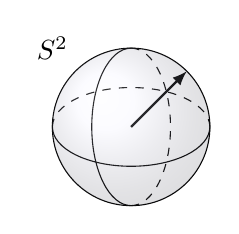
\begin{tikzpicture}
    \draw[->, thick, \select, >=latex] (0,0) -- (45:1cm);
    \draw (-1,0) arc (180:360:1cm and 0.5cm);
    \draw[dashed] (-1,0) arc (180:0:1cm and 0.5cm);
    \draw (0,1) arc (90:270:0.5cm and 1cm);
    \draw[dashed] (0,1) arc (90:-90:0.5cm and 1cm);
    \draw (0,0) circle (1cm);
    \shade[ball color=blue!10!white,opacity=0.20] (0,0) circle (1cm);
    \node at (-1,1) {$S^2$};
  \end{tikzpicture}%
  \caption{We consider three-dimensional spins, \ie{} elements of the unit
  sphere~$S^2$.}
\label{fig:s2}
\end{figure}

\begin{figure}
  \centering
  \begin{tikzpicture}
    \latticeinter{4}
    \begin{scope}[xshift=8cm,yshift=1cm]
      \lattice{4}
    \end{scope}
  \end{tikzpicture}%
  \caption{On the left side we show a two-dimensional spin lattice. Each lattice
  site carries a magnetic moment or spin, represented by an arrow of unit
  length, \ie{}, in the two-dimensional picture, by an element of~$S^1$. The
  neighbors of a lattice site are the ones above, below, left and right in the
  two-dimensional case. The blue squares are the neighbors of the red circle.
  The three-dimensional picture on the right side becomes unclear in a
  two-dimensional drawing rather quickly. Note that the magnetic moments are now
  also three-dimensional, \ie{} elements of the two-dimensional unit
  sphere~$S^2$. In three dimensions each vertex has up to six neighbors.}
\label{fig:lattice}
\end{figure}

We work with a cubic lattice
%
\begin{equation}
  \Sigma := \numlist{1}{N_x} \times \numlist{1}{N_y} \times
  \numlist{1}{N_z} \subset \bN^3 \subset \bR^3\:,
\end{equation}
%
where we interpret~$(i,j,k) \in \Sigma$ as~$i \hx + j \hy + k \hz
\in \bR^3$. Here,~$\hx, \hy, \hz$ are the standard basis vectors of~$\bR^3$.
Note that we can translate the whole lattice by arbitrary integer linear
combinations of the standard basis vectors, thus starting at~$(1,1,1)$ does not
have any physical meaning. It merely corresponds nicely to the numerical
implementation in any~$1$-indexed programming language. At each point~$\r \in
\Sigma$ we attach a spin~$\S_{\r} \in S^2$, which yields the overall
configuration space
%
\begin{equation}
  \Pi := \prod_{\r \in \Sigma} S^2\:.
\end{equation}
%
Each element of~$\Pi$ consists of~$\abs{\Sigma}=N_x N_y N_z$ spins and thus
describes one possible configuration of the whole system. We refer to the
specific spin at position~$\r \in \Sigma$ by~$\S_{\r} \in S^2$. Note that only
the positions of the spins are discretized, but not explicitly their directions.
In any real implementation there is always a fine grained discretization caused
by the finite number of representable floating point numbers. Discrete vertices
and continuous spins mirror nicely the natural crystal structure of solids.

In a typical physical simulation one might want to find the ground state of this
system, \ie{} the lowest energy state, for some given external and internal
parameters. Alternatively, we could be interested in macroscopic properties such
as the specific heat or magnetization. Necessarily, we need to define some
notion of energy and also identify some possible parameters for the spin
lattice. Apparently any physical measure of energy must be based on interactions
between the spins within the system or with external fields. Let us elaborate on
some possible interactions. Each of them comes with a constant that can be
interpreted as a weight, \ie{} how much the respective interaction contributes
to the energy with respect to the others. Those material constants can be
treated as free parameters in the simulation.
%
%%%%%%%%%%%%%%%%%%%%%%%%%%%%%%%%%%%%%%%%%%%%%%%%%%%%%%%%%%%%%%%%%%%%%%%%%%%%%%%%
\section{Interactions}\label{sec:interactions}
%%%%%%%%%%%%%%%%%%%%%%%%%%%%%%%%%%%%%%%%%%%%%%%%%%%%%%%%%%%%%%%%%%%%%%%%%%%%%%%%
%
\subsubsection{Ferromagnetic/direct exchange}

The most obvious interaction is the \newterm{ferromagnetic} or \newterm{direct}
exchange. Pictorially speaking, it favors constellations where spins that are
close to each other point into the same direction. A system only interacting
this way will end up in a state where all spins are parallel to each other. The
measure for parallelism of two neighboring spins~$\S_{\r_1}, \S_{\r_2} \in S^2$
can be expressed as
%
\begin{equation}
  -\S_{\r_1} \cdot \S_{\r_2} =
  -\norm{\S_{\r_1}} \norm{\S_{\r_2}} \cos(\alpha) \:,
\end{equation}
%
where~$\alpha$ is the angle between~$\S_{\r_1}$ and~$\S_{\r_2}$. The minus sign
ensures that the energy of two parallel spins is actually smaller than the
energy of two perpendicular or even antiparallel ones. In the continuum theory
of magnetic moments, the direct exchange term consists of a gradient, which is a
local quantity, \ie{} the gradient at a point only depends on an arbitrarily
small neighborhood of the point. Thus we will always consider the ferromagnetic
exchange to be \newterm{local} or \newterm{short ranged} in the sense that it
only contributes to the energy for adjacent lattice sites, as shown in
\figref{fig:lattice}.

\subsubsection{Interaction with an external field}

Another important and absolutely standard exchange term describes the
interaction of the system with an \newterm{external magnetic field}. Clearly,
every spin tries to align with an external field~$\B$, which we express
mathematically via~$-\B \cdot \S$ for every spin~$\S$ on the lattice. This
contribution is also called the \newterm{Zeeman energy}. It can be misleading to
use terms such as \newterm{non-local} or \newterm{long ranged} for this
exchange, since it is not an interaction between two or more spins within the
system, but affects each lattice site independently in the same fashion.
Naturally, for the external field,~$\B$ itself is the weight or parameter of the
interaction.

\subsubsection{Dipole-dipole interaction}

The \newterm{dipole-dipole interaction} is somewhat more complex, but also much
weaker than the two previous ones. For two spins~$\S_{\r_1}, \S_{\r_2} \in S^2$,
it is given by
%
\begin{equation}
  - {\norm{\r}^{-3}} (3 (\S_{\r_1} \cdot \hat{\r})
  (\S_{\r_2} \cdot \hat{\r}) - \S_{\r_1} \cdot \S_{\r_2})\:,
\end{equation}
%
where~$\r = \r_2 - \r_1$ and~$\hat{\r} = \r / \norm{\r}$ points from the
location of the first spin to the location of the second one. The dipole-dipole
interaction depends on the distance between the two lattice sites as well as the
orientation of the two spins not only relative to each other, but also to the
line connecting them. Moreover, the explicit dependence on the relative position
already indicates that the dipole-dipole interaction is relevant for each pair
of magnetic moments in the system, it is a long ranged interaction. For a
lattice with~$N^3$ vertices the number of pairs scales like~$N^6$. Due to
limited computational resources and its relative weakness, most simulations do
not take the dipole-dipole exchange into account. We will also disregard it
completely in our implementation.

\subsubsection{Dzyaloshinskii-Moriya exchange}

In this work we are interested in certain crystals that lack inversion symmetry,
\eg{} MnSi, and thus exhibit chiral magnets. The missing inversion symmetry
gives rise to the so called \newterm{weak Dzyaloshinskii-Moriya} (DM) coupling.
In the continuum it is described by a term proportional to~$-\S(\r) \cdot
(\nabla \times \S(\r))$. Just like the gradient, the curl of a vector field is a
local property, thus the DM exchange only contributes for adjacent lattice
sites. The discretized version for two spins~$\S_{\r_1}, \S_{\r_2} \in S^2$ at
neighboring positions~$\r_1, \r_2 \in \Sigma$ reads
\begin{equation}
  - (\S_{\r_1} \times \S_{\r_2}) \cdot (\r_2 - \r_1)\:.
\end{equation}
%
Note that~$\r_2 - \r_1$ is normalized by definition for neighboring vertices.
Since the cross product is zero for parallel vectors and maximal for
perpendicular ones, the DM coupling acts against the ferromagnetic interaction
and favors constellations where adjacent spins are perpendicular to each other.
%
%%%%%%%%%%%%%%%%%%%%%%%%%%%%%%%%%%%%%%%%%%%%%%%%%%%%%%%%%%%%%%%%%%%%%%%%%%%%%%%%
\section{The Hamiltonian}\label{sec:hamiltonian}
%%%%%%%%%%%%%%%%%%%%%%%%%%%%%%%%%%%%%%%%%%%%%%%%%%%%%%%%%%%%%%%%%%%%%%%%%%%%%%%%
%
\subsubsection{Summing up the interactions}

Let us now combine the FM and DM interaction as well as an external magnetic
field to compute the energy for the lattice~$\Sigma$. To this end we add up the
contributions from each spin and for each interaction. For instance, the
external field exchange term simply becomes
%
\begin{equation}\label{Bsum}
  -\sum_{\r \in \Sigma} \S_{\r} \cdot \B\:.
\end{equation}
%

Adding up the terms for the FM interaction with all direct neighbors naively as
in
%
\begin{equation}\label{FMsumnaive}
  -\sum_{\r \in \Sigma} \S_{\r} \cdot (\S_{\r + \hx} + \S_{\r - \hx} +
    \S_{\r + \hy} + \S_{\r - \hx} + \S_{\r + \hz} + \S_{\r - \hz})\:,
\end{equation}
%
poses two problems. First, apparently in this fashion we count the interaction
between some pairs of spins multiple times. If~$\Sigma$ was an infinite grid,
\ie{}~$\Sigma=\bZ^3$, we would count every pair exactly twice and could simply
divide~\eqref{FMsumnaive} by~$2$. However,~$\Sigma$ is finite which leads
to the second more subtle issue. Not every lattice site has a neighbor in each
direction~$\hx, \hy, \hz$. Consider the spin in the lower right corner of the
lattice in \figref{fig:lattice}. The sum in our first naive expression for the
FM interaction~\eqref{FMsumnaive} suggests that we need its right and lower
neighbor, which apparently do not exist. As a consequence, we need to define
some behavior at the boundaries. There are several ways to do this and a
plausible treatment of boundary conditions is a central aspect of many different
areas in scientific computing. It is important to realize that this is not
simply an implementation nuisance that we can get rid off by any means that do
not break the code. Various boundary conditions represent different physical
systems and can significantly alter the results of a simulation.

\subsubsection{Boundary conditions}

In many cases the desired simulation volume is an infinite space, or at least so
large compared to all internal length scales that it is practically infinite. On
physical computing machines we are always limited to finite grids. The most
obvious way for finite systems is to set all spins outside of~$\Sigma$ to zero,
\ie{}~$\S_\r = 0$ for all~$\r \in \bZ^3 \setminus \Sigma$. Consequently the
lattice sites on the boundary have less neighbors to interact with. This is
called an \newterm{open boundary}. Open boundaries are often undesirable,
because they heavily impact the physical behavior. In our example, a magnetic
moment at the boundary is less effected by the FM and DM interaction, simply
because it has less neighbors. However, the external field still has the same
impact on a boundary spin as on any other vertex. This imbalance leads to
polarized magnetic moments at the boundaries, \ie{} they tend to all point in
the direction of the external magnetic field~$\B$ to maximize their Zeeman
energy.

One common way to get out of this dilemma is to implement \newterm{periodic
boundary conditions}. We think of our lattice as a finite box of volume~$L^3$
for~$L\in \bRp$ and simply replicate that box infinitely many times to fill the
whole space, see \figref{fig:periodic} for a two-dimensional illustration. In
practice, we will access the lattice sites by indexing a three-dimensional array
with indices~$(i,j,k)\in\Sigma$. Whenever the algorithm tries to index out of
bounds, \eg{} requests~$j=N_y + 1$, we simply use~$j=1$ again. For~$i=0$ we
use~$i=N_x$,~$k=N_z+2$ is replaced by~$k=2$ and so on. In general, this behavior
can be achieved by always working with the indices
%
\begin{equation}\label{periodicindices}
  ((i-1 \mod N_x) + 1, (j-1 \mod N_y) + 1, (k-1 \mod N_z) + 1) \in \Sigma
\end{equation}
%
whenever the algorithm requests the spin at position~$(i,j,k) \in \bZ^3$. By
construction, those new indices always lie in~$\Sigma$. We can now
unproblematically include spins at officially non-existing positions in our
mathematical expressions, implicitly assuming that those are being wrapped
around periodically to positions within the original lattice. This way every
vertex has the same number of neighbors and we do not observe spurious boundary
effects. In this report, we will only employ periodic boundary conditions in all
three directions using~\eqref{periodicindices}. For other scenarios we kept the
possibility of opening up the boundaries in one direction. This solves the issue
of missing neighbors, which we encountered in~\eqref{FMsumnaive}.

\subsubsection{Combining all interactions}

Now that we have established a well defined behavior at the boundary, we can
also tackle the first problem of counting interactions multiple times. For
periodic boundary conditions we could divide the whole expression by~$2$. In the
implementation we do not want to actually carry out redundant computations, thus
we work with
%
\begin{equation}\label{FMsum}
  -\sum_{\r \in \Sigma} \S_{\r} \cdot
    (\S_{\r + \hx} + \S_{\r + \hy} + \S_{\r + \hz})\:.
\end{equation}
%
It is worth convincing oneself that in this expression, assuming open or
periodic boundary conditions, every pair of neighboring lattice sites is
included exactly once.

Finally, the overall DM energy is analogously
%
\begin{equation}\label{DMsum}
  -\sum_{\r \in \Sigma} ((\S_{\r} \times \S_{\r + \hx}) \cdot \hx +
    (\S_{\r} \times \S_{\r + \hy}) \cdot \hy +
    (\S_{\r} \times \S_{\r + \hz}) \cdot \hz)\:.
\end{equation}
%
Everything we discussed about boundary conditions for the FM exchange also holds
true for the DM interaction. Ultimately, adding up all
interactions~\eqref{Bsum},~\eqref{FMsum} and~\eqref{DMsum}, we obtain the
Hamiltonian, \ie{} the energy of the system in a given configuration~$\pi \in
\Pi$
%
\begin{align}\label{hamiltonian}
  H(\pi) = &-\sum_{\r \in \Sigma}\biggl(\S_{\r} \cdot \B +
      J \S_{\r} \cdot (\S_{\r+\hx} + \S_{\r+\hy} + \S_{\r+\hz})\nonumber \\
      &+ K (\S_{\r} \times \S_{\r+\hx} \cdot \hx +
            \S_{\r} \times \S_{\r+\hy} \cdot \hy +
            \S_{\r} \times \S_{\r+\hz} \cdot \hz)\biggr)\:.
\end{align}
%
The parameters~$J$,~$K$ and~$\B$ are sometimes used synonymously for the
ferromagnetic, the Dzyaloshinskii-Moriya and the external field interaction
terms. The physical behavior of the system strongly depends on these freely
adjustable parameters. For a given set of parameters and at zero temperature we
expect the system to settle in the ground state, which can be defined as the
lowest energy configuration
%
\begin{equation}\label{objective}
  \argmin_{\pi \in \Pi} H(\pi)\:.
\end{equation}
%

\subsubsection{Anisotropy}

% While we have remedied the problem of unwanted boundary effects due to missing
% neighbors, we are still working in a finite volume. While any real crystal also
% has a finite volume, it can typically be considered infinite relative to the
% lattice spacing. Due to computational limitations we can only simulate lattices
% with roughly~$30^3$ vertices. Thus the whole lattice is only~$30$ orders of
% magnitudes longer than the lattice spacing which leads to significant
% \newterm{finite size effects}.

In~\eqref{hamiltonian} we have collected all interactions on the lattice. Those
originally stem from a continuous model. Therefore we have to expect
discretization errors. In particular, the transition to a finite cubical
lattice introduces anisotropies that are absent in the original continuum model.
Buhrandt and Fritz show in~\cite{skyrmionlattice} that we can partly compensate
for those disruptive anisotropies by adding next-nearest neighbor interactions
to the Hamiltonian. The optimal choice to render higher order deviations from
the continuous model as small as possible is
%
\begin{align}\label{hamiltonianfix}
  H'(\pi) = & \sum_{\r \in \Sigma} \biggl(
  \frac{J}{16} \S_{\r} \cdot (\S_{\r+2\hx} + \S_{\r+2\hy} + \S_{\r+2\hz})\nonumber \\
  &+ \frac{K}{8} (\S_{\r} \times \S_{\r+2\hx} \cdot \hx +
        \S_{\r} \times \S_{\r+2\hy} \cdot \hy +
        \S_{\r} \times \S_{\r+2\hz} \cdot \hz)\biggr)\:.
\end{align}
%
The Hamiltonian used in the simulation is then~$H + H'$. Note that~$H'$ has the
same structure of the FM and DM term of~$H$, but enters with smaller constants
and opposite sign. Thus it complements the nearest neighbor exchange by a
directly related next-nearest neighbor interaction term. Adding next-nearest
neighbor interactions makes a big difference computationally, but is handled
analogously to the nearest neighbor interactions, see \figref{fig:interact}.
Periodic and open boundaries still work precisely the same way and are already
taken care of by~\eqref{periodicindices}.

\begin{figure}
  \centering
  \begin{tikzpicture}
    \latticeinternn{5}
  \end{tikzpicture}%
  \caption{We select a spin at position~$\r \in \Sigma$ (red circle) and show
  its nearest neighbors as blue squares and the next-nearest neighbors as green
  pentagons. Note that although the diagonally adjacent vertices are closer
  to~$\r$ than the next-nearest neighbors, they are not included in any
  exchange terms of the Hamiltonian.}
\label{fig:interact}
\end{figure}

\subsection{A note on parameter values}

Recall that there is a great conflict of interest between the FM and the DM
interactions. While the FM term in the Hamiltonian is minimal when all spins are
parallel to each other, the DM term favors a configuration where neighboring
spins are orthogonal. The specific compromise between those effects depends
mostly on their respective strengths~$J$ and~$K$. In reality the direct
interaction~$J$ is much stronger and one typically encounters helical structures
with long modulation periods. For example in MnSi the spins wind around a given
modulation axis only once per roughly~$40$ lattice spacings.  By tuning the
ratio~$J/K$ we can set the periodicity. For a period of~$N$ lattice sites, we
have to set~$J/K$ to~$1/\tan(2\pi / N)$. In all our simulations we chose~$J=1$
and~$K=\tan(2\pi / 10)$, \ie{} one full modulation every~$10$ vertices.
Because~$K=\tan(2\pi / 10)\approx 0.73$ is not much smaller than~$J=1$ we cannot
directly model known chiral magnets such as MnSi in our simulation. However,
larger periodicities would require much larger grids and thus be computationally
infeasible. Moreover, we let the external magnetic field point in the~$\hz$
direction~$\B=(0,0,B)$ and only keep~$B$ as a free scalar parameter.

We can fix one of the parameters, in this case~$J$, arbitrarily and then work in
abstract lattice units. A computer can only deal with dimensionless numbers and
in numerical simulations one often makes some convenient, but arbitrary choices.
It is then sometimes quite difficult to translate the results back to physically
meaningful values.

The alert reader might have realized that so far our model does not contain any
thermal energy. When talking about magnetism, temperature typically has a strong
influence on the physical properties of various materials. However, thermal
energy cannot be accounted for by an additional term in the Hamiltonian. Our
intuition tells us that thermal energy is intrinsically of dynamic nature, thus
cannot be captured sensibly in a single static spin configuration. Thermodynamic
observables are statistical properties of an ever evolving underlying system. In
fact we will account for temperature not in the Hamiltonian buy via the
Metropolis algorithm, which we will encounter in \secref{sec:metropolis}, where
the dynamic and statistical nature of thermodynamics will become apparent.

\subsection{Summary}

In this section we have set up our model, which we want to briefly summarize. We
work on the lattice
%
\begin{equation}
  \Sigma := \numlist{1}{N_x} \times \numlist{1}{N_y} \times
  \numlist{1}{N_z} \subset \bN^3 \subset \bR^3\:
\end{equation}
%
and attach a spin~$\S_{\r} \in S^2$ to each lattice site~$\r \in \Sigma$. This
yields the configuration space
%
\begin{equation}
  \Pi := \prod_{\r \in \Sigma} S^2\:.
\end{equation}
%
On~$\Pi$ we define the Hamiltonian~$H+H'$ from~\eqref{hamiltonion}
and~\eqref{hamiltonianfull} where we implement periodic (or partially open)
boundary conditions. The parameters~$J=1$ and~$K=\tan(2\pi / 10)$ of the FM and
DM interaction are fixed, which leaves us only with the magnetic field in
the~$\hz$ direction~$B$ as a free parameter. In the next section we will
introduce the temperature as a second adjustable quantity. Instead of finding
the energy minimizing configuration as stated in~\eqref{objective} at zero
temperature, we now seek to evaluate prominent observables such as the
magnetization or specific heat of the system for given values of~$B$ and~$T$. As
mentioned before, we cannot expect to compute such macroscopic properties from a
single static configuration~$\pi \in \Pi$ due to thermal effects. Before we go
into statistical physics, let us present a first primer on general Monte Carlo
methods.
%
%%%%%%%%%%%%%%%%%%%%%%%%%%%%%%%%%%%%%%%%%%%%%%%%%%%%%%%%%%%%%%%%%%%%%%%%%%%%%%%%
\section{Observables and Analysis}\label{sec:analysis}
%%%%%%%%%%%%%%%%%%%%%%%%%%%%%%%%%%%%%%%%%%%%%%%%%%%%%%%%%%%%%%%%%%%%%%%%%%%%%%%%
%
